\documentclass[]{book}
\usepackage{lmodern}
\usepackage{amssymb,amsmath}
\usepackage{ifxetex,ifluatex}
\usepackage{fixltx2e} % provides \textsubscript
\ifnum 0\ifxetex 1\fi\ifluatex 1\fi=0 % if pdftex
  \usepackage[T1]{fontenc}
  \usepackage[utf8]{inputenc}
\else % if luatex or xelatex
  \ifxetex
    \usepackage{mathspec}
  \else
    \usepackage{fontspec}
  \fi
  \defaultfontfeatures{Ligatures=TeX,Scale=MatchLowercase}
\fi
% use upquote if available, for straight quotes in verbatim environments
\IfFileExists{upquote.sty}{\usepackage{upquote}}{}
% use microtype if available
\IfFileExists{microtype.sty}{%
\usepackage{microtype}
\UseMicrotypeSet[protrusion]{basicmath} % disable protrusion for tt fonts
}{}
\usepackage[margin=1in]{geometry}
\usepackage{hyperref}
\hypersetup{unicode=true,
            pdftitle={Angewandte Statistische Methoden in den Nutztierwissenschaften},
            pdfauthor={Peter von Rohr},
            pdfborder={0 0 0},
            breaklinks=true}
\urlstyle{same}  % don't use monospace font for urls
\usepackage{natbib}
\bibliographystyle{apalike}
\usepackage{longtable,booktabs}
\usepackage{graphicx,grffile}
\makeatletter
\def\maxwidth{\ifdim\Gin@nat@width>\linewidth\linewidth\else\Gin@nat@width\fi}
\def\maxheight{\ifdim\Gin@nat@height>\textheight\textheight\else\Gin@nat@height\fi}
\makeatother
% Scale images if necessary, so that they will not overflow the page
% margins by default, and it is still possible to overwrite the defaults
% using explicit options in \includegraphics[width, height, ...]{}
\setkeys{Gin}{width=\maxwidth,height=\maxheight,keepaspectratio}
\IfFileExists{parskip.sty}{%
\usepackage{parskip}
}{% else
\setlength{\parindent}{0pt}
\setlength{\parskip}{6pt plus 2pt minus 1pt}
}
\setlength{\emergencystretch}{3em}  % prevent overfull lines
\providecommand{\tightlist}{%
  \setlength{\itemsep}{0pt}\setlength{\parskip}{0pt}}
\setcounter{secnumdepth}{5}
% Redefines (sub)paragraphs to behave more like sections
\ifx\paragraph\undefined\else
\let\oldparagraph\paragraph
\renewcommand{\paragraph}[1]{\oldparagraph{#1}\mbox{}}
\fi
\ifx\subparagraph\undefined\else
\let\oldsubparagraph\subparagraph
\renewcommand{\subparagraph}[1]{\oldsubparagraph{#1}\mbox{}}
\fi

%%% Use protect on footnotes to avoid problems with footnotes in titles
\let\rmarkdownfootnote\footnote%
\def\footnote{\protect\rmarkdownfootnote}

%%% Change title format to be more compact
\usepackage{titling}

% Create subtitle command for use in maketitle
\newcommand{\subtitle}[1]{
  \posttitle{
    \begin{center}\large#1\end{center}
    }
}

\setlength{\droptitle}{-2em}
  \title{Angewandte Statistische Methoden in den Nutztierwissenschaften}
  \pretitle{\vspace{\droptitle}\centering\huge}
  \posttitle{\par}
  \author{Peter von Rohr}
  \preauthor{\centering\large\emph}
  \postauthor{\par}
  \predate{\centering\large\emph}
  \postdate{\par}
  \date{2017-02-26}

\usepackage{booktabs}
\usepackage{amsthm}
\makeatletter
\def\thm@space@setup{%
  \thm@preskip=8pt plus 2pt minus 4pt
  \thm@postskip=\thm@preskip
}
\makeatother

\begin{document}
\maketitle

{
\setcounter{tocdepth}{1}
\tableofcontents
}
\chapter*{Vorwort}\label{vorwort}
\addcontentsline{toc}{chapter}{Vorwort}

Dieses Dokument umfasst die kompletten Unterlagen zur Vorlesung
\textbf{Angewandte Statistische Methoden in den Nutztierwissenschaften}.
Der Titel dieser Vorlesung ist sehr allgemein gehalten. Dies würde es
erlauben einen grosszügigen Überblick über eine breite Palette an
statistischen Methoden, welche in den Nutztierwissenschaften eingesetzt
werden, zu geben.

Wir schlagen an dieser Stelle aber einen anderen Weg ein, und
fokussieren uns auf die statistischen Methoden in der genomischen
Selektion. Nur diese bewusste Wahl eines spezifischen Gebietes
ermöglicht es uns, den behandelten Stoff angemessen zu vertiefen. Im
anschliessenden Unterabschnitt wollen wir die hier getroffene
Entscheidung der Fokusierung auf die genomische Selektion motivieren.
Dabei wird klar, dass wir mit der Wahl des Themas der multiplen linearen
Regression als Ausgangspunkt auch eine Leserschaft ansprechen, welche
nicht primär an der Tierzucht interessiert ist.

\section*{Motivation}\label{motivation}
\addcontentsline{toc}{section}{Motivation}

Vom Standpunkt der statistischen Modellierung, ist das einfache lineare
Modell mit fixen Effektstufen für den Einsatz in der genomischen
Selektion ausreichend. Diese Art von Modellen werden auch als
Regressionsmodelle bezeichnet. Die Problematik entsteht erst bei der
Technik, welche wir für die Schätzung der unbekannten Parameter
verwenden können. In der klassischen Regressionsanalyse ist die Methode
der kleinsten Quadrate (Least Squares) die Methode der Wahl. Least
Squares können wir aber für die genomische Selektion nicht verwenden, da
die Anzahl unbekannter Parameter (\(p\)) grösser ist als die Anzahl
Beobachtungen (\(n\)).

Mit der steigenden Grösse und Komplexität von aktuellen Datensätzen
tritt das soeben beschriebene Problem nicht nur in der Tierzucht auf,
sondern es gibt eine breite Palette von Anwendungen. In der Vorlesung
beschrieben wir diese Problematik am Beispiel der genomischen Selektion
und es werden alternative Techniken zur Schätzung von Parametern
vorgeschlagen. Da die Methode der multiplen Regressionsanalyse in
früheren Vorlesungen behandelt wurde, bietet diese ein idealer
Ausgangspunkt für den in dieser Veranstaltung präsentierten Stoffinhalt.

\section*{Einordnung}\label{einordnung}
\addcontentsline{toc}{section}{Einordnung}

Die Vorlesung \textbf{Angewandte Statistische Methoden in den
Nutztierwissenschaften} ist eine halb-semestrige Veranstaltung und wird
im Masterstudiengang Agrarwissenschaften der ETH Zürich angeboten.

\section*{Lernziele}\label{lernziele}
\addcontentsline{toc}{section}{Lernziele}

Für die Verwendung des hier präsentierten Stoffs schlagen wir die
folgenden Lernziele vor.

Die Studierenden \ldots{}

\begin{itemize}
\tightlist
\item
  kennen die Eigenschaften der multiplen linearen Regression und
\item
  können einfache Datensätze mithilfe der Regressionsmethode analysieren
\item
  wissen wieso multiple lineare Regressionen bei der genomischen
  Selektion nicht brauchbar ist
\item
  kennen die in der genomischen Selektion verwendeten statistischen
  Verfahren, wie

  \begin{itemize}
  \tightlist
  \item
    BLUP-basierte Verfahren,
  \item
    Bayes'sche Verfahren und
  \item
    die LASSO Methode
  \end{itemize}
\item
  können einfache Übungsbeispiele mit der Statistiksoftware R
  erfolgreich bearbeiten.
\end{itemize}

\chapter{Einführung}\label{intro}

Den in dieser Vorlesung präsentierte Stoff kann aus mehreren
Gesichtspunkten betrachtet werden. Aus Sicht der Tierzucht behandeln wir
die statistischen Methoden, welche in der \textbf{genomischen Selektion}
angewendet werden. Für Statistiker stellen wir verschiedene Methoden der
Regularisierung in hoch-parametrischen Modellen vor. In der sehr
populären Disziplin des \textbf{Machine Learnings} wird das hier
besprochene Problem als die Selektion von relevanten Features im Kontext
des Supervised Learnings dargestellt.

\section{Beschreibung des Problems}\label{problem}

Alle die soeben genannten Formulierungen beschreiben das gleiche
Problem. Wir gehen von einem Datensatz aus, welcher aus Beobachtungen
besteht. Jede Beobachtung ist charakterisiert durch sehr viele
unabhängige Grössen. Die Gewichtung der zu einer Beobachtung gehörenden
Grössen wird über unbekannte Parameter erreicht.

Als Beispiel für einen solchen Datensatz können wir eine Population mit
SNP-typisierten Tieren betrachten. Das Typisierrungsergebnis für ein
bestimmtes Tier enthält die Genotypen an den Genorten, welche bei der
Typisierung untersucht werden. Die einzelnen Genorte werden als
sogenannte Single Nucleotide Polymorphisms (SNP) bezeichnet. In
Abhängigkeit des anbietenden Labors gibt es verschiedene Optionen für
die gewünschte Typisierung. Die Optionen unterscheiden sich vor allem in
der Dichte der untersuchten Genorte. Das heisst bei einer grösseren
Dichte werden mehr SNPs untersucht. Typische Werte von gängigen
Anbietern bewegen sich im Bereich zwischen 50000 (50K) bis rund 800000
(800K) untersuchte SNPs pro untersuchtes Genom. Die totale Anzahl an SNP
im Genom beträgt rund 20 Millionen. Somit ist ein Typisierungsergebnis
eine vom Anbieter gemachte Auswahl aller verfügbaren SNPs.

\section{Rückblick}\label{background}

Bis Anfangs des 21. Jahrhundert wurden eigentlich keine genomischen
Informationen in Zuchtprogrammen berücksichtigt. Mit genomischer
Information ist hier die Genotyp-Varianten einer grosser Anzahl von
Genorten, welche über das ganze Genom verteilt ist. Um die
Jahrtausendwende waren sehr viele ForscherInnen in einem Gebiet aktiv,
welches damals als Mapping von sogenannten
\texttt{Quatitative\ Trait\ Loci} (QTL) bezeichnet wurde. Eine Übersicht
zu QTL ist im Buch \citep{BBC2008}. Das Ziel der Untersuchungen im
Bereich QTL-Mapping war das Finden von Regionen im Genom, welche wichtig
sind für die Ausprägung von spezifischen Phänotypen. Heute spricht man
nicht mehr QTL-Mapping sondern heute wird die Suche von genetischen
Orten, welche einen wichtigen Einfluss auf die Ausprägung eines
Phänotyps haben, mit \texttt{Genome\ Wide\ Association\ Study} (GWAS)
bezeichnet.

Trotz umfangreicher Forschungstätigkeit auf dem Gebiet des QTL-Mappings,
fanden keine Resultate aus diesen Arbeiten den Weg in die praktische
Zuchtarbeit. Somit verläuft die Zuchtarbeit bis vor kurzem nach dem
klassischen Schema, welches nachfolgend gezeigt ist.

\begin{center}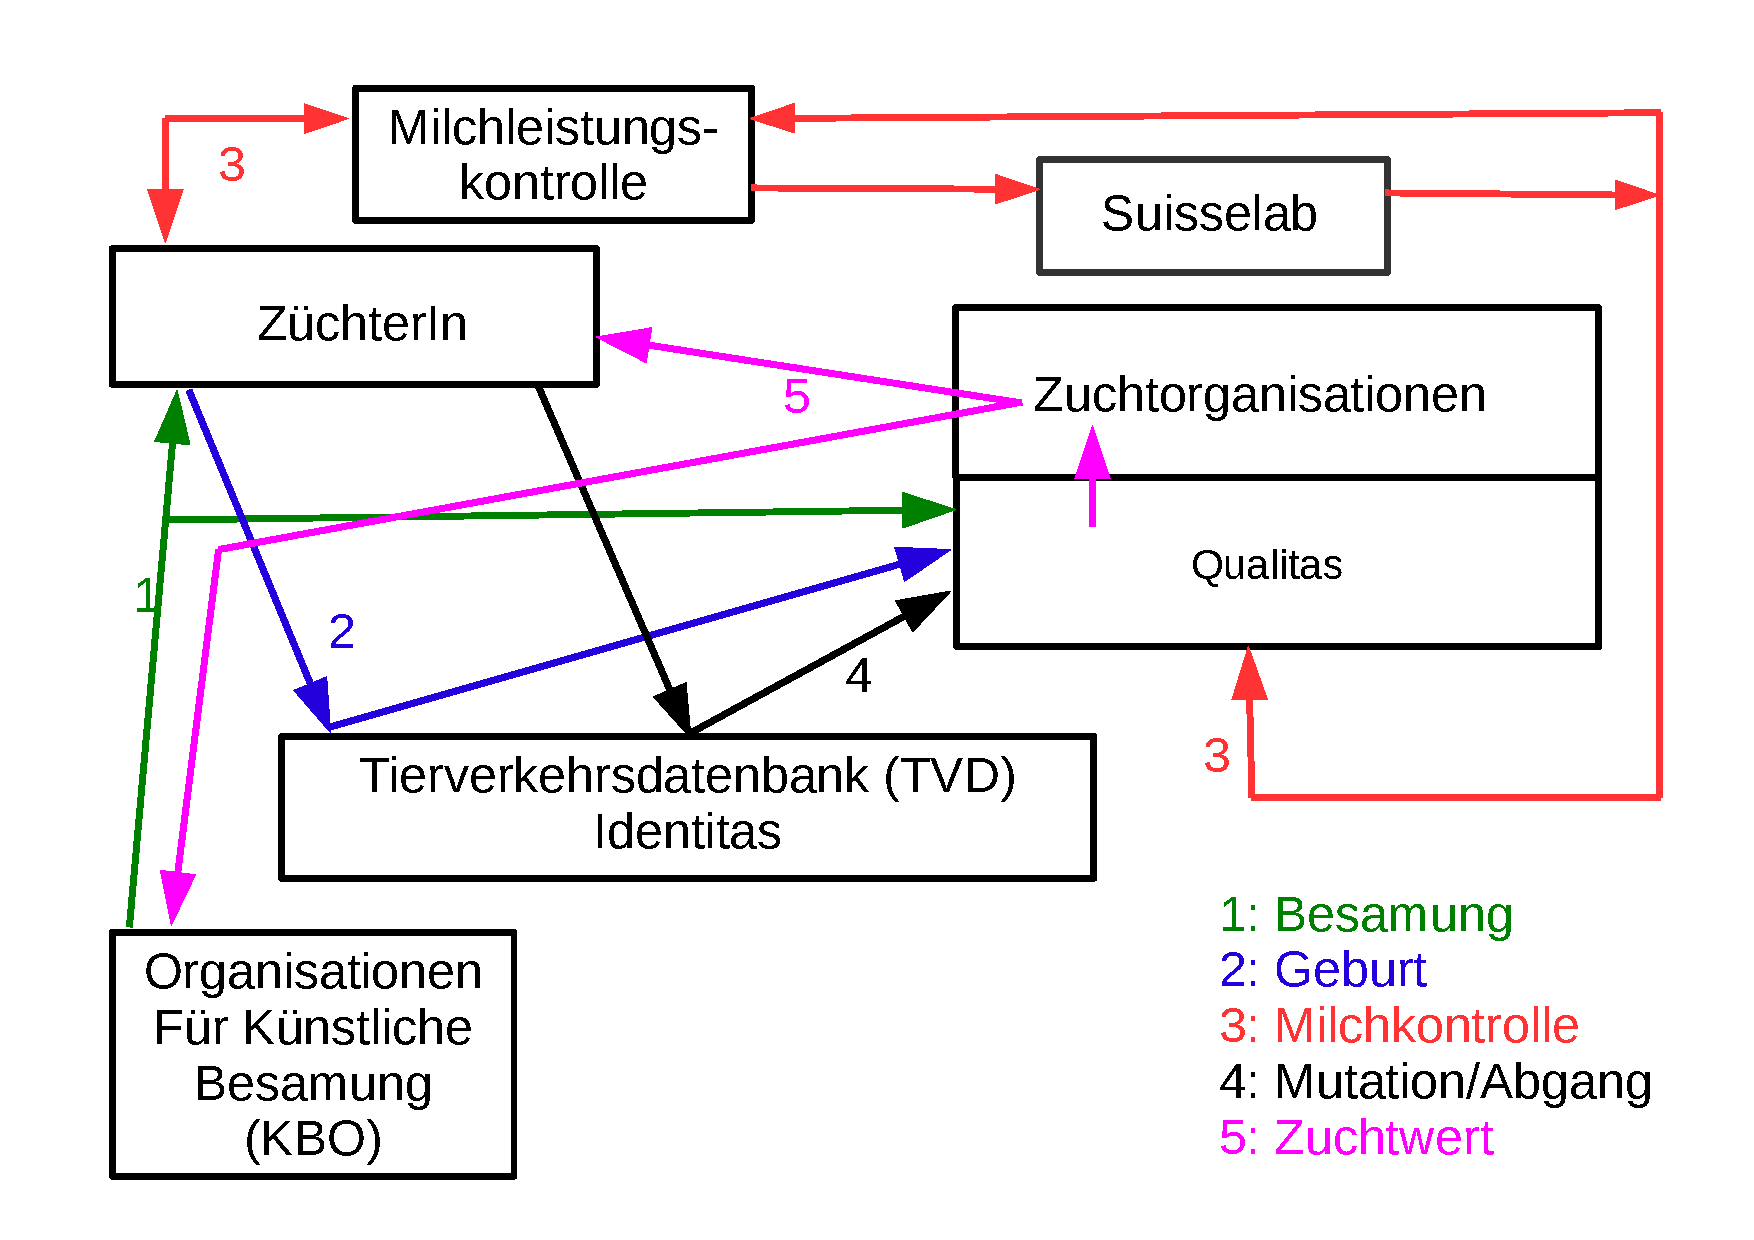
\includegraphics{ZuchtprogrammKomplett} \end{center}

\subsection{Paradigmenwechsel}\label{paradigmenwechsel}

Die Publikation \citep{MHG2001} gilt als Grundstein für eine neue Ära in
der praktischen Zuchtarbeit. Die Autoren haben gezeigt, wie genomische
Information, welche in genügender Dichte vorliegen muss, zur Schätzung
von Zuchtwerten verwendet werden kann. Sie konnten auch statistische
Methoden zeigen, mit welchen die Parameter in verwendeten Modell
geschätzt werden können. Wir werden zu einem späteren Zeitpunkt noch
genauer auf den Inhalt des Papers von \citep{MHG2001} zurückkommen.

\subsection{Vor der genomischen
Selektion}\label{vor-der-genomischen-selektion}

Von Anfangs der 1980-er Jahre wurden die statistischen Auswertungen in
den Zuchtprogrammen auf das BLUP-Tiermodell abgestellt. In dieser Zeit
wurden die einfachen Modelle auch durch verschiedene Erweiterungen
ausgebaut. Bei der Milchproduktion wurde von einfachen
Laktationsleistungen auf Testtagesmodelle umgestellt. Bei der Wurfgrösse
beim Schwein oder anderen diskreten Merkmalen wurden auch
\texttt{Generalized\ Linear\ Mixed\ Models} (GLMM) verwendet. Unabhängig
von den verwendeten Modellen wurden in allen Auswertungen die gleichen
Informationen berücksichtigt. - phänotypische Leistungen - Pedigree -
Varianzkomponenten aus periodischen Schätzungen

Versuchsweise wurde ab den 1990-er Jahren erste genetische Marker mit in
den Zuchtprogrammen berücksichtigt. Das Problem war dass diese wenigen
Markern sehr schnell auf einer bestimmten Variante fixiert war. Nach der
Fixierung lieferten diese Genorte keine zusätzliche Information zur
Auswahl von potentiellen Zuchttieren. Es war zu dieser Zeit nicht klar,
wie das Problem der Fixierung von einzelnen Genorten behandelt werden
soll und es gab auch keine wirklich gute Strategie für die
Berücksichtigung von genetischen Informationen in Zuchtprogrammen.

\subsection{Modellierung vor der genomischen
Selektion}\label{modellierung-vor-der-genomischen-selektion}

Vor der Einführung der genomischen Selektion war das BLUP-Tiermodell die
Methode der Wahl für die Auswertung von Leistungsdaten in der Tierzucht.
In seiner einfachsten Form sieht dieses Modell wie folgt aus.

\begin{equation}
  y = Xb + Zu + e
\end{equation}

\begin{tabular}{lll} 
wobei  &  $y$  &  Vektor mit phänotypischen Beobachtungen\\ 
       &  $b$  & Vektor mit fixen Effekten              \\ 
       &  $X$  & Inzidenzmatrix, welche fixe Effekte den Beobachtungen zuordnet\\ 
       &  $u$  & Vektor mit Zuchtwerten (zufällig) \\ 
       &  $Z$  & Inzidenzmatrix der Zuchtwerte \\ 
       &  $e$  & Vektor mit Residuen (zufällig) 
\end{tabular}

Die Co-Varianzen der zufälligen Komponenten sind definiert als:

\[Var(\mathbf{e}) = \mathbf{R} = \mathbf{I}*\sigma_e^2\]
\[Var(\mathbf{u}) = \mathbf{G} = \mathbf{A} * \sigma_g^2\]
\[Cov(\mathbf{u},\mathbf{e}^T) = Cov(\mathbf{e}, \mathbf{u}^T) = \mathbf{0}\]
\[\rightarrow Var(\mathbf{y}) = \mathbf{V} = \mathbf{ZGZ}^T + \mathbf{R}\]

\section{Genomische Selektion}\label{gensel}

Vom Standpunkt der Genetik aus basiert das BLUP-Tiermodell auf dem
sogenannten Infinitesimalmodell. In diesem Modell wird angenommen, dass
die phänotypische Ausprägung eines Merkmals durch die Summe von
unendlich vielen Genorten mit undendlich kleiner Wirkung verursacht
wird. Durch diese Annahme lässt sich dem einzelnen Tier kein fix
definierter Genotyp mehr zuordnen. Diese fehlende Zuordnung der
einzelnen Genotypen wird über die Modellierung der Zuchtwerte als
zufällige Effekte gelöst. Die zufälligen Effekte der Zuchtwerte
entsprechen dabei Realisierungen einer Zufallsvariablen mit vorgegebener
Verteilung.

In der genomischen Selektion verwenden wir das polygene Modell. Dabei
werden die phänotypischen Leistungen als Summe von bekannten Genorten
zusammengesetzt. Die konkrete Umsetzung des polygenen Modells wurde zum
ersten Mal im Paper von \citep{MHG2001} gezeigt. Diese Autoren haben
aufgrund von simulierten Daten gezeigt, dass es mit Hilfe einer sehr
dichten Markerkarte möglich ist, die phänotypischen Leistungen alleine
aufgrund der geschätzten Wirkungen an den Markergenorten zu modellieren.

Die folgende Abbildung fasst die Unterschiede zwischen dem
Infinitesimalmodell und dem polygenen Modell zusammen.

\begin{center}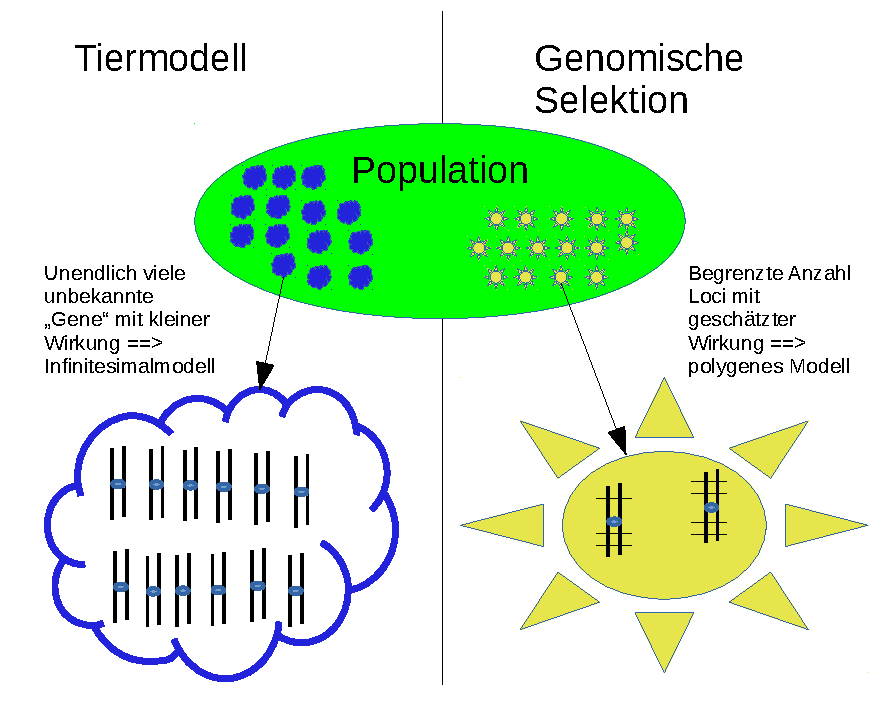
\includegraphics{AnimalModelVsGenomicSelection} \end{center}

\subsection{Modellierung}\label{modellierung}

Im Zusammenhang mit der genomischen Selektion besteht die Modellierung
der Daten aus zwei Komponenten

\begin{enumerate}
\def\labelenumi{\arabic{enumi}.}
\tightlist
\item
  Die Schätzung der Gen-Wirkungseffekte (\(a\))
\item
  Die Schätzung der genomischen Zuchtwerte
\end{enumerate}

Die Umsetzung der beiden Komponenten wird in zwei verschiedenen
Verfahren gemacht. Im Zwei-Schritt-Verfahren werden beide Komponenten
einzeln an verschiedenen Teilen der Zuchtpopulation ausgeführt. Im
Gegensatz dazu werden im Single-Step-Verfahren beide Komponenten im
gleichen Schritt realisiert.

\subsection{Zwei-Schritt-Verfahren}\label{zwei-schritt-verfahren}

Beim Zwei-Schritt-Verfahren wird die Population in ein Trainings- und
ein Testset unterteilt. Im Trainingsset werden aufgrund von
Typisierungsergebnissen und Beobachtungen die Gen-Wrkungseffekte (\(a\))
geschätzt. Sobald die Schätzwerte für die \(a\)-Effekte bekannt sind
können diese für die Schätzung der genomischen Zuchtwerte verwendet
werden.

Da aufgrund der Typisierungsergebnisse die Genotypen an den SNP-Genorten
bekannt sind, brauchen wir kein gemischtes lineares Modell mehr. Im
Gegensatz zur BLUP-Zuchtwertschätzung, ist in der genomischen Selektion
beim Zwei-Schritt-Verfahren ein einfaches lineares Modell ausreichend.
Im Idealfall, wenn die komplette Information zu allen
Gen-Wirkungseffekten (\(a\)) bekannt sind, dann setzen sich die
genotypischen Werte einfach zusammen aus den aufsummierten \(a\)-Werten.
In Matrix-Vektor-Schreibweise können wir die folgende Modellgleichung
aufstellen.

\begin{equation}
  g = 1\mu + Ma + \epsilon
\end{equation}

\begin{tabular}{lll}
wobei:  &  $g$         &  Vektor von wahren genomischen Zuchtwerten \\
        &  $\mu$       &  Achsenabschnitt \\
        &  $a$         &  Vektor mit Gensubstitutionseffekten \\
        &  $M$         &  Inzidenzmatrix als Verknüpfung zwischen $a$ und $g$ \\
        &  $\epsilon$  &  Vektor von zufälligen Residuen 
\end{tabular}

Die Matrix \(M\) ist eine Inzidenzmatrix, welche die genotypischen Werte
im Vektor \(g\) mit den Gen-Wirkungseffekten \(a\) verknüpft. Die Matrix
\(M\) hat die Dimension \(n\times p\) wobei \(n\) der Anzahl Individuen
mit einem Typisierungsergebnis entspricht und \(p\) gleich der Anzahl
SNP-Genorte ist.

In der Realität im ersten Schritt des Zwei-Schritt-Verfahrens kennen wir
aber weder die Komponenten des Vektors \(g\) noch die
Gensubstitutionseffekte \(a\). Somit müssen wir das Modell zur Schätzung
der \(a\)-Effekte modifizieren. Bei der aktuellen Modifikation ersetzen
wir den Vektor \(g\) durch die phänotypischen Beobachtung \(y\).

\begin{equation}
  y = (1\mu + Xb) + Ma + (\epsilon+ e)
\end{equation}

\begin{tabular}{lll}
wobei:  &  $y$  &  Vektor der phänotypischen Beobachtungen \\
        &  $b$  &  Vektor der fixen Umweltfaktoren \\
        &  $X$  &  Inzidenzmatrix der fixen Effekte\\
        &  $e$  &  Vektor von nicht-genetische Residuen
\end{tabular}

Das Modell mit den phänotypischen Beobachtungen erlaubt eine Schätzung
der \(a\)-Effekte. Mit diesem Ansatz gibt es aber zwei Probleme.

\begin{enumerate}
\def\labelenumi{\arabic{enumi}.}
\tightlist
\item
  \textbf{Verfügbarkeit}: wirtschaftliche Merkmale wie Milchleistung
  sind nur beim weiblichen Geschlecht beobachtbar. Somit müsste für die
  Selektion auf der männlichen Seite wieder auf Nachkommenleistungen
  zurückgegriffen werden. Dies verlängert aber das
  Generationenintervall.
\item
  \textbf{Vergleichbarkeit}: Beim Austausch von Information zwischen
  verschiedenen Ländern sind die phänotypischen Leistungen nicht
  unbedingt vergleichbar.
\end{enumerate}

Diese beiden Probleme können gelöst werden, wenn anstelle von
phänotypischen Leistungen \(y\), geschätzte Zuchtwerte \(\hat{g}\)
verwendet werden. Das entsprechende Modell sieht dann wie folgt aus.

\begin{equation}
\hat{g} = g + (\hat{g} - g) = 1\mu + Ma + (\epsilon + (\hat{g} - g) )
\end{equation}

\subsection{Eigenschaften von
BLUP-Zuchtwerten}\label{eigenschaften-von-blup-zuchtwerten}

Aufgrund der Eigenschaften von den BLUP-Zuchtwerten \(\hat{g}\) führt
die Addition der Abweichung \((\hat{g} - g)\) zu einer Reduktion der
Varianz. Die Reduktion der Varianz bedeutet, dass
\(var(\hat{g}) \le var(g)\) ist. Für BLUP-Zuchtwerte gilt, dass die
Covarianz zwischen wahrem und geschätztem Zuchtwert gleich der Varianz
der geschätzten Zuchtwerte ist. In Formeln geschrieben bedeutet dass,

\begin{equation}
  cov(\hat{g},g) = var(\hat{g})
\end{equation}

Setzen wir diese Beziehung in die Varianz der Abweichung
\((\hat{g} - g)\) ein, dann erhalten wir

\begin{equation}
  var(\hat{g} - g) = var(\hat{g}) + var(g) - 2cov(\hat{g},g) = var(g) - var(\hat{g}) \ge 0
\end{equation}

Somit gilt, dass \(var(g) \ge var(\hat{g})\) und somit ist die Reduktion
der Varianz gezeigt. Im Zusammenhang mit der Varianzreduktion steht auch
die zweite Eigenschaft von BLUP-Zuchtwerten, welche uns hier
Schwierigkeiten bereitet und zwar handelt es sich dabei um den
sogenannten Shrinkage-Effekt. Für einen geschätzten Zuchtwert eines
Tieres \(i\) bedeutet das, dass dieser zum Durchschnitt der geschätzten
Zuchtwerte der Eltern regressiert wird. Das Ausmass dieses
Regressions-Effektes hängt davon ab, aufgrund welcher Informationen der
Zuchtwert von Tier \(i\) geschätzt wurde. Diese Abhängigkeit wird in der
Zerlegung des geschätzten BLUP-Zuchtwertes des Tieres \(i\) in seine
Komponenten sichtbar. Diese Zerlegung ist in \citep{Hofer1990} und in
\citep{vonRohr2016} erklärt. Das Resultat der Zerlegung ist in der
nachfolgenden Formel zusammengefasst.

\begin{eqnarray}
\hat{g}_i &=& \frac{1}{1 + \alpha \delta^{(i)} + {\alpha\over 4} \sum_{j=1}^n \delta^{(k_j)}}
              \left[y_i - \hat{\mu} + {\alpha\over 2}\left\{\delta^{(i)}(\hat{g}_s + \hat{g}_d) 
              + \sum_{j=1}^n \delta^{(k_j)} (\hat{g}_{k_j} - {1\over 2}\hat{g}_{l_j}) \right\} \right]
\label{eq:AhatDecompEq}
\end{eqnarray}

Die Zerlegung des geschätzen Zuchtwertes \(\hat{g}_i\) für Tier \(i\)
zeigt die Abhängigkeit des Ausmasses der Regression von \(\hat{g}_i\)
auf den Durchschnitt der geschätzten Elternzuchtwerte \(\hat{g}_s\) und
\(\hat{g}_d\). Hat das Tier \(i\) keine Eigenleistung \(y_i\), keine
Nachkommen und keine Paarungspartner, so ist \(\hat{g}_i\) vollständig
durch \(\hat{g}_s\) und \(\hat{g}_d\) bestimmt. Sobald aber Tier \(i\)
eine Eigenleistung hat und später dann noch Nachkommenleistungen
dazukommen, nimmt der Einfluss von \(\hat{g}_s\) und \(\hat{g}_d\) auf
\(\hat{g}_i\) ab. Damit verringert sich auch das Ausmass des
Regressions-Effektes von \(\hat{g}_i\) auf den Durchschnitt der
geschätzten Elternzuchtwerte.

Durch die Berücksichtigung zusätzlicher Informationen, wie Eigenleistung
und Leistungen von Nachkommen und Paarungsparter, bei der Schätzung des
Zuchtwertes für Tier \(i\) steigt auch die Genauigkeit oder das
Bestimmtheitsmass (\(B\)) des geschätzten Zuchtwertes. Wir können
aufgrund der Eigenschaften von BLUP-Zuchtwerten können wir folgende
Zusammenhänge aufstellen. Je grösser die verfügbare Information für die
Schätzung eines Zuchtwertes für Tier \(i\), desto grösser ist das
Bestimmtheitsmass des geschätzten Zuchtwertes und je tiefer ist der
Regressions-Effekt des geschätzten Zuchtwertes auf den Durchschnitt der
geschätzten Zuchtwerte der Eltern und je geringer ist auch die
Varianzreduktion.

\subsection{Einsatz von BLUP-Zuchtwerten in der genomischen
Selektion}\label{einsatz-von-blup-zuchtwerten-in-der-genomischen-selektion}

Eigenschaften von BLUP-Zuchtwerten führen zu Varianzreduktion und dazu
dass geschätzte Zuchtwerte zum Durchschnitt der geschätzten Zuchtwerte
der Eltern regressiert werden. Diese beiden Effekte sind problematisch
bei der Verwendung von BLUP-Zuchtwerten für die Schätzung der
\(a\)-Effekte in der genomischen Selektion. Ein bestimmtes Tier \(i\)
hat immer die gleichen SNP-Genotypen und wir gehen davon aus, dass diese
auch immer die gleiche Wirkung auf die Ausprägung eines Phänotyps haben.
Der mit BLUP geschätzte Zuchtwert eines Tieres ändert sich aber während
seines Lebens. In der Zeitperiode der Geburt bis zur Beobachtung einer
Eigenleistung ist der geschätzte Zuchtwert durch die geschätzten
Zuchtwerte der Eltern bestimmt. Mit zunehmendem Alter werden für Tier
\(i\) mehr Informationen in der Zuchtwertschätzung berücksichtigt. Somit
ändert sich der geschätzte Zuchtwert und damit würde sich auch die
aufgrund der BLUP-Zuchtwerte geschätzten \(a\)-Effekte ändern. Das ist
aufgrund von unserer Annahme der konstanten Wirkung der \(a\)-Effekte
ein unerwünschtes Verhalten.

Die unerwünschten Veränderungen der geschätzten BLUP-Zuchtwerte werden
durch eine Prozedur namens \textbf{Deregression} korrigiert. Da sich die
Veränderungen der Zuchtwerte im wesentlichen durch eine Funktion der
Änderungen im Bestimmtheitsmass beschrieben werden kann, ist die
Deregression als Korrektur von geschätzten Zuchtwerten aufgrund deren
Bestimmtheitsmass definiert. Einzelheiten zur Deregression können dem
Paper \citep{GTF2009} entnommen werden.

\section{Zusammenfassung}\label{zusammenfassung}

Die deregressierten Zuchtwerten werden als Beobachtunen für die
Schätzung der \(a\)-Effekte im ersten Schritt des
Zwei-Schritt-Verfahrens verwendet. Die geschätzen \(a\)-Werte werden
dann verwendet um im zweiten Schritt die genomischen Zuchtwerte der
restlichen Population zu berechnen.

Die im Zwei-Schritt-Verfahren verwendeten Modelle zur Schätzung der
\(a\)-Effekte sind einfache lineare Modelle. Die Anzahl der Parameter
\(p\) in diesen Modellen entspricht der Anzahl zu schätzender
\(a\)-Werte und somit der Anzahl an SNPs pro Typisierung. Diese Anzahl
ist typischerweise bei 50K kann aber auch bis 800K anwachsen. In den
meisten Fällen ist \(p >> n\), wenn \(n\) die Anzahl typisierter Tiere
ist. Somit können wir das klassische Least Squares Verfahren für die
Schätztung der Parameter nicht verwenden.

\section{Ausblick}\label{ausblick}

Das Problem \(p >> n\) kommt heutzutage in sehr vielen Anwendungen vor.
In den nachfolgenden Kapiteln wollen wir uns ein paar Lösungsansätze
anschauen, welche uns trotz der spärlich verfügbaren Informationen in
den hoch-dimensionalen Parameterräumen, sinnvolle Schätzwerte für die
Parameter im Modell liefern kann.

\chapter*{Abkürzungen}\label{abkurzungen}
\addcontentsline{toc}{chapter}{Abkürzungen}

\begin{tabular}{l|l}
\hline
Abbreviation & Meaning\\
\hline
QTL & Quatitative Trait Loci\\
\hline
GWAS & Genome Wide Association Study\\
\hline
GLMM & Generalized Linear Mixed Models\\
\hline
\end{tabular}

\bibliography{ASMNW.bib}


\end{document}
